\chapter{Introduction}
\section{Overview of Steam Drum Control}

Industrial Boiler systems are used for many purposes, from supplying steam to various locations like hospitals to propulsion systems to the more common power generation. Boilers are now operating at higher pressure and are being built smaller than they were, and causes faster process control responses \cite{controlguruWebsite}. Because of high pressure operation, boilers must have an adequate level of control to stay safe. Due to the phenomena of minimum phase behavior and the shrink and swell effect, the boiler drum level control initially reacts in direct opposition to what is required for process stability. Shrink and swell refers to a phenomenon that when the drum pressure drops, some water in the tubes flashes, and those steam bubbles push water in the tubes above them up into the drum, temporarily raising the drum level. Then when the system stabilizes and those steam bubbles either collapse or reach the drum, the tubes rapidly refill with water from the drum, dropping its level. The effect is asymmetrical - when drum pressure rises due to falling steam demand, it temporarily suppresses the production of steam in the tubes but the effect is more subtle. \cite{crossco} This effect must then be accounted for if the system is to be properly controlled.  A Drum Boiler Schematic can be seen in Figure \ref{fig:schematic}.

% When the drum pressure drops, some water down in the tubes flashes, and those steam bubbles push water in the tubes above them up into the drum, raising the drum level even as the total mass of water in the drum and tubes falls.

\begin{figure}[ht]
    \begin{center}
    \resizebox{\ScaleModelImage \textwidth}{!}{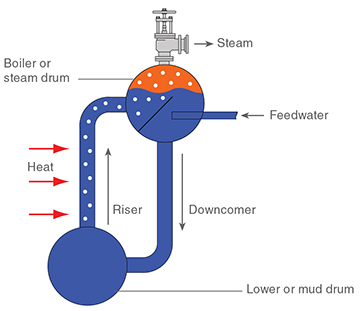
\includegraphics{Graphics/Graphic.png}}
    \caption{Drum Boiler Schematic \cite{spiraxsarcoWebsite}}
    \label{fig:schematic}
    \end{center}
\end{figure}

\section{Literature Review}


Mathematical models for a Boiler-Tubine system exist in the literature, however most are simplified to not include the dynamics of the drum's water level nor the shrink and swell effect. The model developed by \r{A}str\"{o}m and Bell \cite{Astrom} provides sufficient detail to model these parameters.
An extension of this model was developed by Iacob and Andreescu \cite{Iacob} which provides modeling for the feed-water valve, fuel flow valve, steam valve, throttle pressure, and power output. 

Steam boiler is a highly nonlinear system which poses significant complexities in its control system design and analysis.  Conventional control method is known as {\it three element control} in the industry, which is effectively a PID type control system that regulates three measured quantities in the boiler, such as liquid level in the drum, feed water flow, and steam flow leaving the drum.  The three-element control is based on linearized dynamics of the boiler that provides the required boiler performance when the deviation of the state variables remains relatively small with respect to the nominal state.  This research investigates design of boiler control system that is expected to provide a better system performance when large variations of the system state may occur.



\section{Goals and Objectives of proposed research}

%%% Section 1.3 needs some narrative rather than bullet points.  Typically the outline should be
%%% a) the goals of the research
%%% b) scope of the research/methodology

The broad objective of this research is to develop a control system that provides the desired performance of the steam boiler for a wider range of its operating state.  Conventional three-element control or other linear control methods which rely on linearized model of the boiler have limited performance as the boiler must operate near the nominal operating point of the system.  This research explores the application of the Model Predictive Control (MPC) for the design of the boiler control system.  In recent years, MPC control method has found significant attention in industry \cite{Wang, Forbes, Zang, Botelho} and academia \cite{Saltık, Ghosh, Song} alike with excellent performance.  There are several advantages of the MPC control system that make it an ideal candidate for its application to the boiler control, such as 1) it does not require that the system operate near a nominal operating point, 2) it is easy to include various constraints in the control design, and 3) it is possible to design a controller even when the system model is not precisely known.

The goals of this thesis are

\begin{itemize}
  \item Review mathematical model of the steam boiler
  \item Investigate limitations of conventional control systems, such as PID and LQR
  \item Apply model predictive control system to the steam boiler and analyze its performance
\end{itemize}

The developed control system will be evaluated by simulation only as there are no experimental facilities are available.  For the mathematical model of the boiler, we will consider the \r{A}str\"{o}m and Bell \cite{Astrom} model which is quite well known in the literature.  The closed loop system will be analyzed in Matlab/Simulink environment under various operating conditions. 

\section{Outline of the Thesis}

This following is an outline of the rest of this thesis proposal: Chapter 2 presents the basics of the three-element control and the LQR control which will be followed by details of Model Predictive Control design method.  In Chapter 3 we present the \r{A}str\"{o}m and Bell \cite{Astrom} model of the steam boiler and the model validation.  Chapter 4 presents some simulation results of three-element control and the LQR control.  Chapter 5 outlines plans for further research on application of MPC control and conclusions. 


